\chapter{Implementácia}
\label{kap:implementacia} % id kapitoly pre prikaz ref

\section{Implementačný jazyk}

Backend aplikácie pracuje v jazyku Java. Keďže potrebujeme vytvoriť REST API, na ktoré bude možné posielať requesty z frontendu, na túto úlohu využijeme Spring Boot. Knižnicou, ktorú sme si vybrali pre prácu s RDF dátami v jazyku Java je Apache Jena. Tvorí ju viacero častí, ktoré spolu , pričom kľúčové časti pre našu aplikáciu sme uviedli vo východiskovej kapitole (\ref{secJena}).   

Frontend aplikácie je tvorený v knižnici React, ktorý patrí medzi najrýchlejšie frameworky vo svojej kategórii, najmä kvôli tomu, že ak dôjde k zmene vlastností nejakého vnoreného komponentu, nie je nutné prepočítavať a znovu vykresľovať všetky nadradené komponenty, ale zmeny sa vykonajú iba v tých komponentoch, v ktorých je to nevyhnutné. Na jednoduché dizajnovanie komponentov je využitá knižnica Bootstrap. Pri vytváraní formulárov je použitá knižnica Formik, ktorá uľahčuje prácu s formulármi v Reacte a zároveň je možné ju použiť s Yup, čo je nástroj na vytváranie validačnej schémy pre JavaScript, a teda je jednoduchšie kontrolovať vstup od používateľa.

\section{Správa stavu frontendu aplikácie}
Celá webová aplikácia sa v Reacte skladá z komponentov. V prípade ak potrebujeme medzi komponentmi vzájomne komunikovať je to možné zabezpečiť pomocou parametrov. Posielať si všetky informácie v parametroch však nie je vždy jednoduché, najmä v prípade, ak všetky komponenty nie sú hierarchicky usporiadané je potrebné medzi dvoma komponentami na jednej úrovni zdielať rovnakú informáciu. Pre jednoduchšie a prehľadnejšie spravovanie stavu celej aplikácie sme vuyžili Redux.  

\begin{figure}[h]
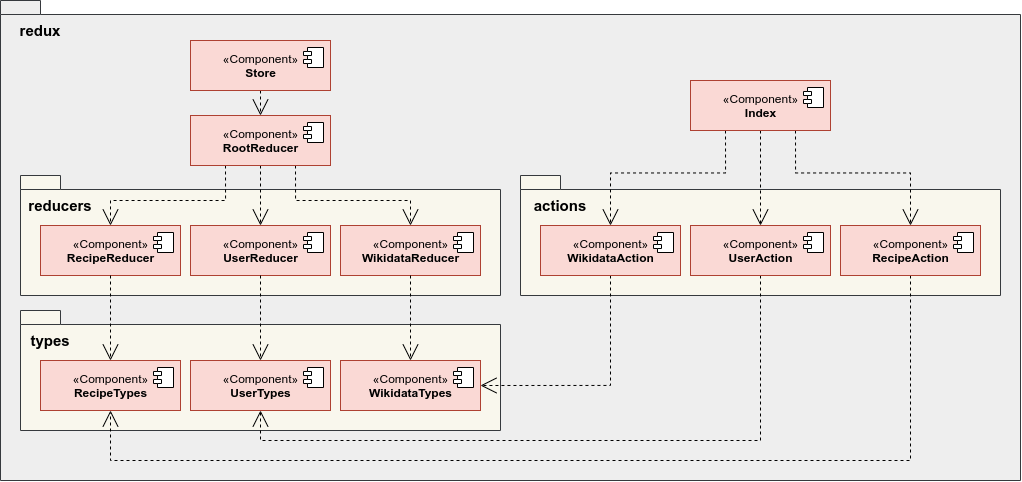
\includegraphics[width=\textwidth]{images/reactRedux}
\caption{Vizualizácia štruktúry balíčkov a súborov pracujúcich so stavom aplikácie}
\label{reactRedux}
\end{figure}

Ako vidíme na obr. \ref{reactRedux}, balíček redux je rozdelený do 3 ďalších balíčkov, pričom každý z týchto balíčkov obsahuje práve 3 súbory. Je to z toho dôvodu, že každý zodpovedá za jednu z častí aplikácie, teda za používateľa (za prihlásenie, informácie o ňom), recepty (jednotlivé filtre, ktoré je možné nastaviť, zoznam práve zobrazených receptov, detail o recepte) alebo za informácie o triedach z wikidata, ktoré sú súčasťou receptov. V balíčku types sú konštanty, konkrétne sú to typy akcií, ktoré sú volané, aby zmenili stav aplikácie. V balíčku reducers, obsahuje každý reducer, čo je funkcia s parametrami, obsahuje definíciu toho, aká zmena má v stave nastať v prípade, ak dôjde k niektorému z typov akcií, ktoré sú zadefinované v balíčku types. Všetky reducery sú skombinované do jedného hlavného reducera, ktorý je následne použitý v súbore Store. Tento súbor vytvára akýsi "sklad" všetkých informácií, ktorý môže čítať akýkoľvek komponent z aplikácie. V balíčku actions sú akcie, ktorými ako jedinými môžeme meniť stav aplikácie z nejakého komponentu, pričom tieto akcie sú všetky dostupné z jediného súboru index v balíčku redux. 

Keďže potrebujeme dispatch-ovať (spúšťať) aj asynchrónne akcie, v našom prípade konrétne pri volaní REST API, využívame aj redux-thunk. 

Stav aplikácie ostáva zachovaný iba do času, kým nedôjde k znovu načítaniu stránky alebo presmerovaniu na inú stránku aplikácie. To spôsobuje problém napr. pri prihlásení používateľa, pričom pri prechode na novú stránku sa stav, ktorý si zachovával informáciu o používateľovi, vynuluje. Z toho dôvodu sme museli využiť local storage, ktorá si informácie o používateľovi dokáže uchovať aj pri prepínaní sa medzi stránkami. 

\section{Prepojenie frontendu, backendu a databázy}
Každá z častí, ktorú sme popísali v časti Návrh (kap. \ref{kap:navrh}) je samostatným komponentom. Požadovanú funkcionalitu však bude celá aplikácia plniť len v prípade, že všetky komponenty budú vzájomne prepojené. Toto prepojenie je zachytené na diagrame z obr. \ref{prepojenieAplikacie}.   

\begin{figure}[h]
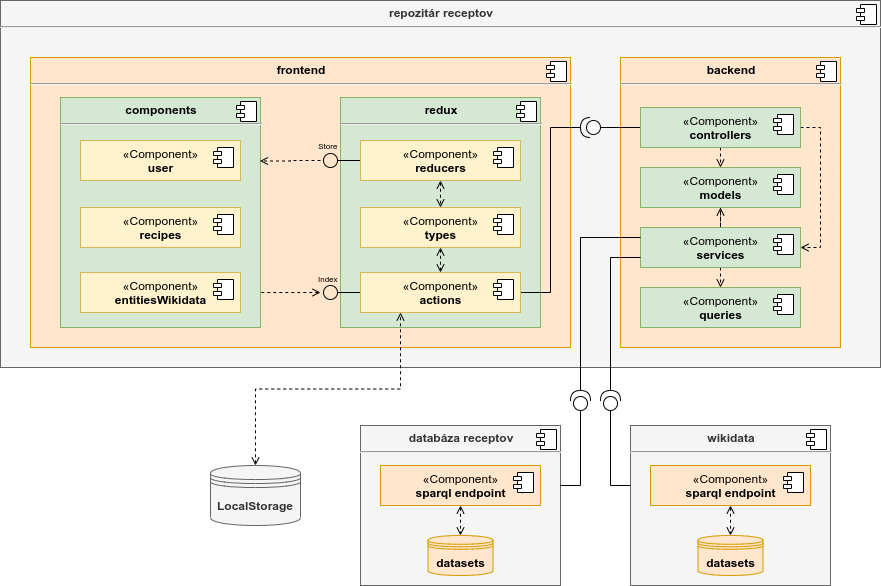
\includegraphics[width=\textwidth]{images/prepojenieComponentDiagram}
\caption{Diagram vyjadrujúci prepojenie jednotlivých častí aplikácie}
\label{prepojenieAplikacie}
\end{figure}

Frontend posiela pomocou knižnice axios requesty na backend. Tieto requesty sú posielané z balíčka actions v reduxe. Na strane backendu sú tieto requesty spracovávané v balíčku controllers, v ktorom metódy obsluhujú URL adresy pre jednotlivé requesty. Odpovede, ktoré tieto metódy posielajú vo forme JSON sú získavané z databázy. S databázou komunikujú iba metódy balíčka services. Tie vytvárajú dopyty, ktoré sú posielané na sparql endpointy pomocou triedy RDFConnection, ktorá je súčasťou Apache Jena. Sparql endpoint potrebný pre našu aplikáciu poskytuje stránka wikidata a zároveň server Apache Fuseki, ktorý nám poskytuje triplestore, v ktorom si udržujeme dáta o receptoch, ktoré sme vytvorili. 
